\documentclass{scrartcl}

\usepackage{amssymb}
\usepackage{amsmath}
\usepackage{tikz}
\usetikzlibrary{decorations.shapes}

%from Foucault - The Order of Things: An Archaeology of the Human Sciences, pp. 80 & 219

\begin{document}
	
	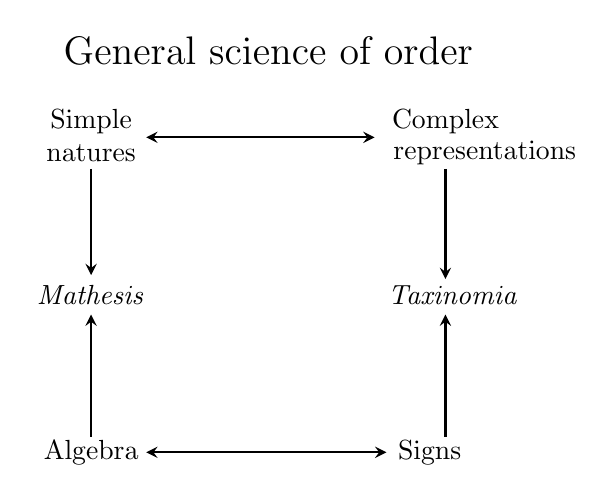
\begin{tikzpicture}[>=stealth]
	\node at (0,3.1) 	 {\Large{General science of order}};
	\node at (-2.25,2.2) {Simple};
	\node at (-2.25,1.8) {natures};
	\node at (-2.25,0) 	 {\textit{Mathesis}};
	\node at (-2.25,-2)  {Algebra};
	\node at (2.25,2.2)  {Complex};
	\node at (2.75,1.8)  {representations};
	\node at (2.35,0) 	 {\textit{Taxinomia}};
	\node at (2.05,-2)	 {Signs};
	
	\draw[<->,thick] (-1.55,2)--(1.35,2);		%simple--complex
	\draw[<->,thick] (-1.55,-2)--(1.5,-2);		%algebra--signs
	%
	\draw[->,thick] (-2.25,1.6)--(-2.25,0.25);		%simple--math
	\draw[->,thick] (-2.25,-1.8)--(-2.25,-0.25);	%algebra--math
	\draw[->,thick] (2.25,1.6)--(2.25,0.2);			%complex--tax
	\draw[->,thick] (2.25,-1.8)--(2.25,-0.25);		%signs--tax
	\end{tikzpicture}
	
		%closer to original diagram, but ugly as shit
	%	\begin{tikzpicture}[>=stealth]
	%	\node at (0,2.75) 		{\Large{General science of order}};
	%	\node at (-3,1.7) 	{Simple};
	%	\node at (-3,1.3) 	{natures};
	%	\node at (-3,0) 	{\textit{mathesis}};
	%	\node at (-3,-1.5) 	{Algebra};
	%	\node at (3,1.7) 	{Complex};
	%	\node at (3.5,1.3) 	{representations};
	%	\node at (3.1,0) 	{\textit{Taxinomia}};
	%	\node at (2.8,-1.5)	{Signs};
	%	
	%	\draw[<->,thick] (-2.3,1.5)--(2.1,1.5);		%simple--complex
	%	\draw[<->,thick] (-2.3,-1.5)--(2.25,-1.5);	%algebra--signs
	%	%
	%	\draw[->,thick] (-3,1.1)--(-3,0.25);		%simple--math
	%	\draw[->,thick] (-3,-1.2)--(-3,-0.25);		%algebra--math
	%	\draw[->,thick] (3,1.1)--(3,0.2);			%complex--tax
	%	\draw[->,thick] (3,-1.2)--(3,-0.25);		%signs--tax
	%	\end{tikzpicture}
	
	
	\vspace{2.5cm}
	
	
	%\begin{figure}
	%	\centering
	\hspace{-2cm}
	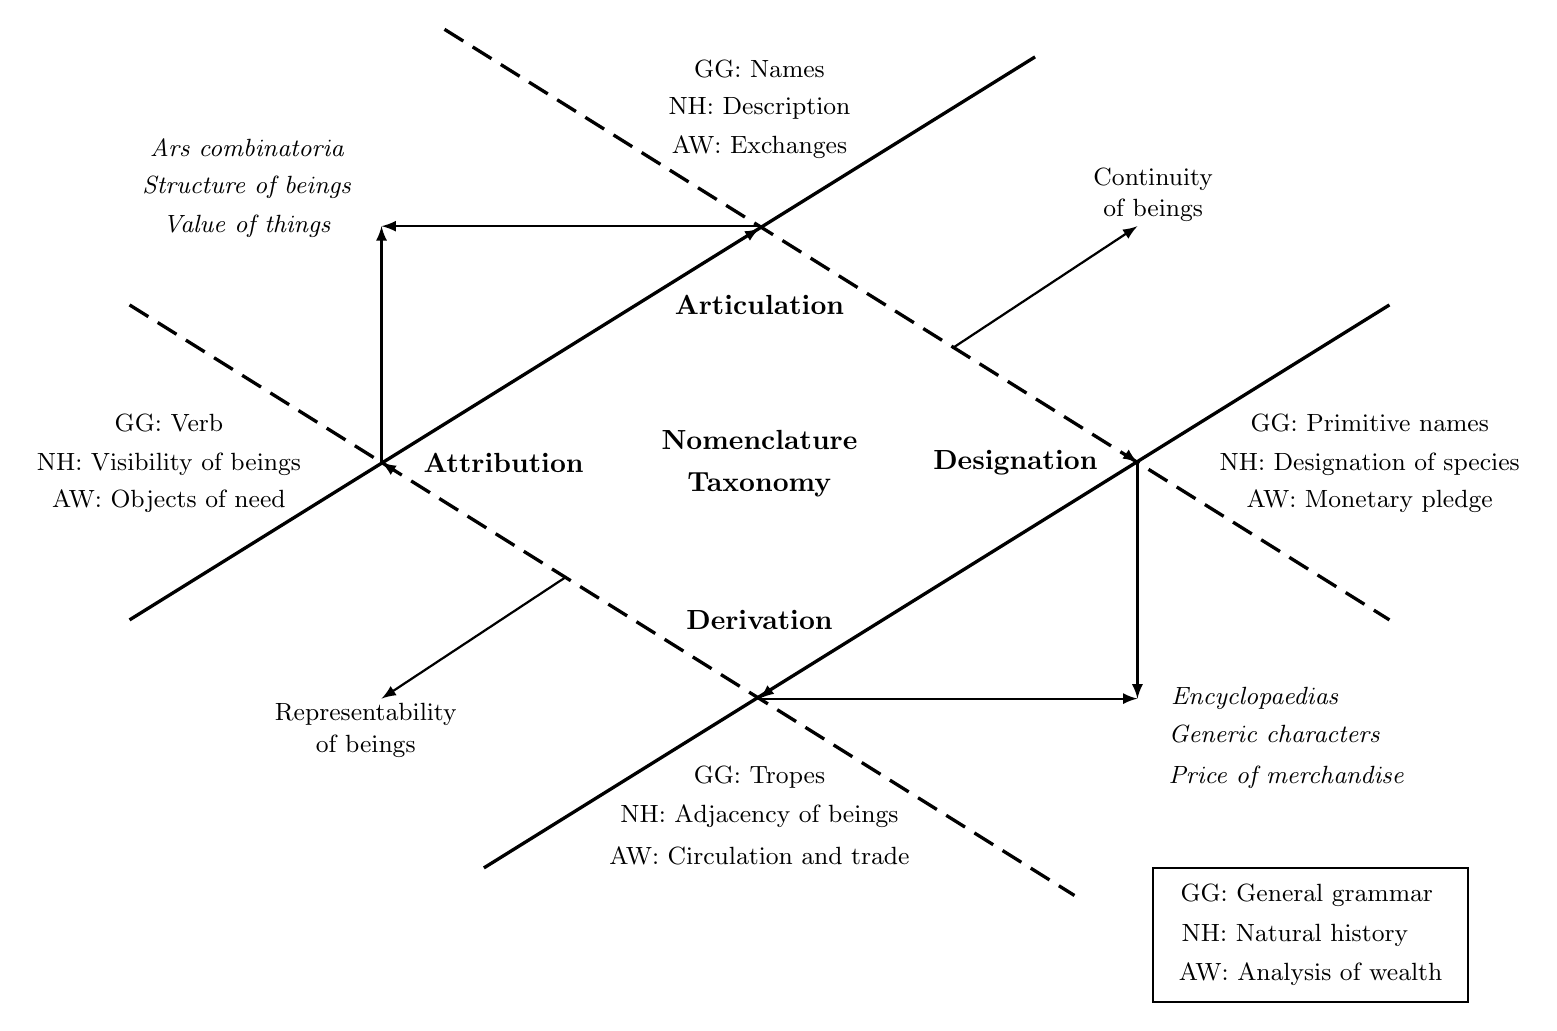
\begin{tikzpicture}
	%inner labels
	\node at (0,2) 	  {\textbf{Articulation}};
	\node at (-3.25,0){\textbf{Attribution}};
	\node at (0,0.28) {\textbf{Nomenclature}};
	\node at (0,-.28) {\textbf{Taxonomy}};
	\node at (3.25,0) {\textbf{Designation}};
	\node at (0,-2)   {\textbf{Derivation}};
	
	%lines
	\draw[very thick] (-8,-2)--(3.5,5.15);		%top NE line
	\draw[very thick] (-3.5,-5.15)--(8,2);		%bottom NE line
	\draw[very thick, dash pattern=on 8pt off 4pt] (-4,5.5)--(8,-2);	%top SE line
	\draw[very thick, dash pattern=on 8pt off 4pt] (-8,2)--(4,-5.5);	%bottom SE line
	
	%arrows
	\draw[->,>=latex,thick] (4.8,0)--(4.8,-3);	%right part, down arrow
	\draw[->,>=latex,thick] (0,-3)--(4.8,-3);	%down part, right arrow
	%
	\draw[->,>=latex,thick] (-4.8,0)--(-4.8,3);	%left part, up arrow
	\draw[->,>=latex,thick] (0,3)--(-4.8,3);	%up part, left arrow
	%
	\draw[->,>=latex,thick] (2.45,1.45)--(4.8,3);		%upper NE diagonal
	\draw[->,>=latex,thick] (-2.45,-1.45)--(-4.8,-3);	%lower SW diagonal
	
	%outer labels
	\node at (0,5)  {\small GG: Names};
	\node at (0,4.5){\small NH: Description};
	\node at (0,4)  {\small AW: Exchanges};
	%
	\node at (-7.5,0.5) {\small GG: Verb};
	\node at (-7.5,-.02){\small NH: Visibility of beings};
	\node at (-7.5,-.5) {\small AW: Objects of need};
	%
	\node at (7.75,0.5) {\small GG: Primitive names};
	\node at (7.75,-.02){\small NH: Designation of species};
	\node at (7.75,-.5) {\small AW: Monetary pledge};
	%
	\node at (0,-4)  {\small GG: Tropes};
	\node at (0,-4.5){\small NH: Adjacency of beings};
	\node at (0,-5)  {\small AW: Circulation and trade};
	%
	\node at (-5,-3.2){\small Representability};
	\node at (-5,-3.6){\small of beings};
	\node at (5,3.6)  {\small Continuity};
	\node at (5,3.2)  {\small of beings};
	%
	\node at (-6.5,4) 	{\textit{\small Ars combinatoria}};
	\node at (-6.5,3.5)	{\textit{\small Structure of beings}};
	\node at (-6.5,3) 	{\textit{\small Value of things}};
	%
	\node at (6.3,-3) 	 {\textit{\small Encyclopaedias}};
	\node at (6.55,-3.45){\textit{\small Generic characters}};
	\node at (6.7,-4) 	 {\textit{\small Price of merchandise}};
	
	%manual arrowheads
	\draw[->,>=latex,thick] (-4.79,-0.0065)--(-4.8,0);	%attrib
	\draw[->,>=latex,thick] (-0.1,2.91)--(0,2.97);		%artic
	\draw[->,>=latex,thick] (0.1,-2.92)--(0,-3);		%deriv
	\draw[->,>=latex,thick] (4.7,0.07)--(4.8,0);		%desig
	
	%legend
	\draw[thick] (5,-5.15) rectangle (9,-6.85);
	\node at (6.95,-5.5) {\small GG: General grammar};
	\node at (6.8,-6)  	 {\small NH: Natural history};
	\node at (7.0,-6.5)  {\small AW: Analysis of wealth};
	%\draw[help lines] (-8,-6) grid (8,6);
	\end{tikzpicture}
	%	\caption{Seventeenth and Eighteenth Centuries}
	%\end{figure}
	
	
	\vspace{1cm}
	
	
	%\begin{figure}
	%	\centering
	\hspace{-2cm}
	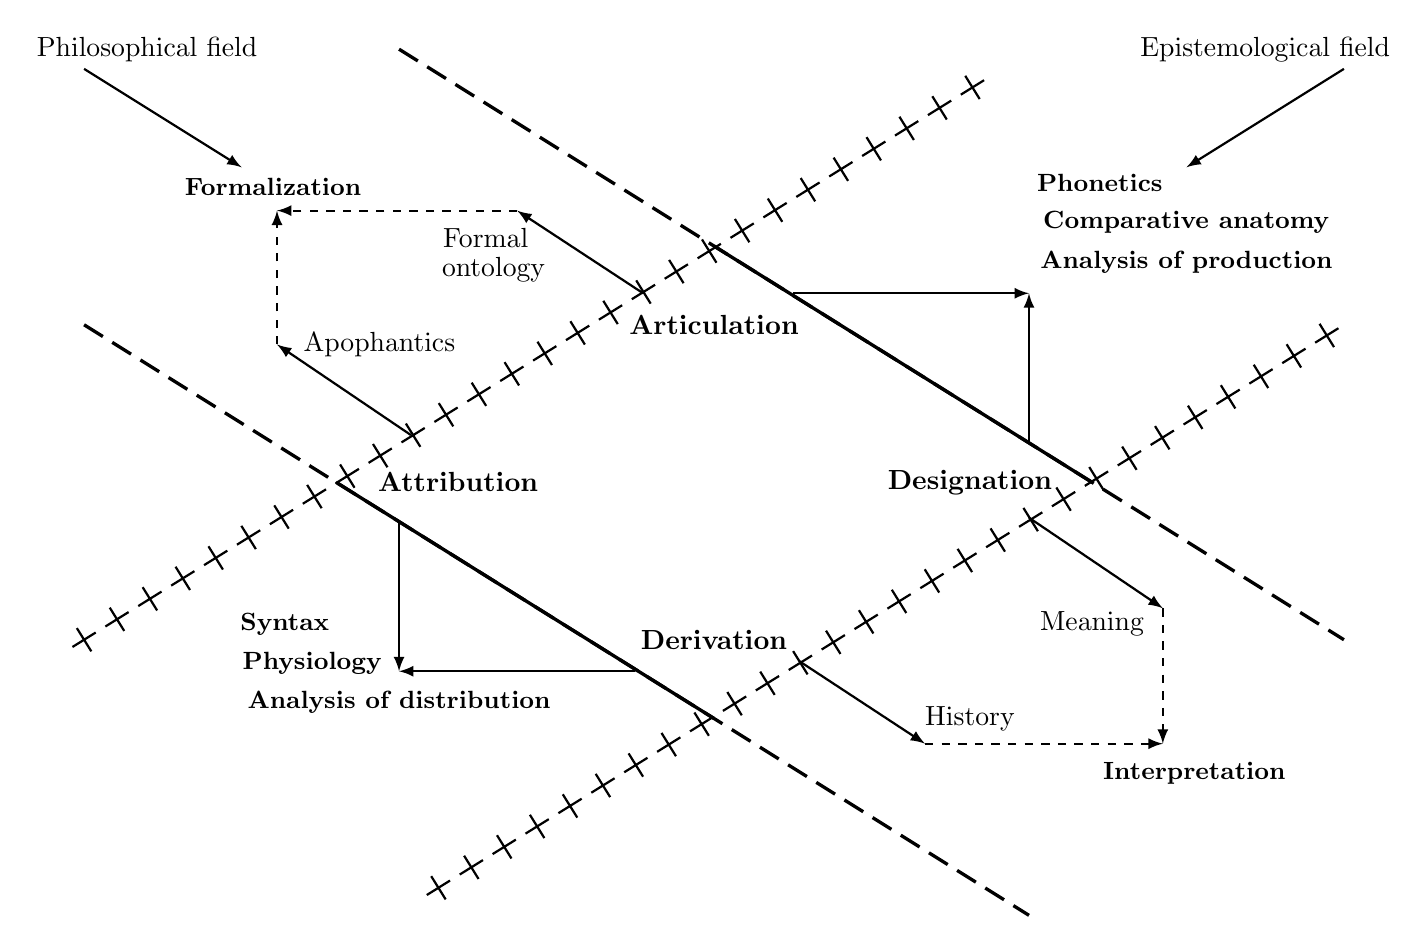
\begin{tikzpicture}
	%inner labels
	\node at (0,2) 	  {\textbf{Articulation}};
	\node at (-3.25,0){\textbf{Attribution}};
	\node at (3.25,0) {\textbf{Designation}};
	\node at (0,-2)   {\textbf{Derivation}};
	
	%lines
	\draw[decorate,decoration={crosses,shape size=7pt,transform={rotate=45},segment length=14pt},thick] (-8,-2)--(3.5,5.15);	%top NE line
	\draw[decorate,decoration={crosses,shape size=7pt,transform={rotate=45},segment length=14pt},thick] (-3.5,-5.15)--(8,2); %bottom NE line
	\draw[very thick, dash pattern=on 8pt off 4pt] (-4,5.5)--(8,-2);	%top SE line
		\draw[very thick] (0,3)--(4.8,0);
	\draw[very thick, dash pattern=on 8pt off 4pt] (-8,2)--(4,-5.5);	%bottom SE line
		\draw[very thick] (0,-3)--(-4.8,0);
		
	%top left part
	\draw[->,>=latex,thick] (-0.9,2.4)--(-2.5,3.45);		%artic
	\draw[->,>=latex,thick] (-3.85,0.6)--(-5.55,1.75);		%attrib
	\draw[->,>=latex,thick,dashed] (-2.5,3.45)--(-5.55,3.45);
	\draw[->,>=latex,thick,dashed] (-5.55,1.75)--(-5.55,3.45);
	\node at (-2.9,3.1) {Formal};
	\node at (-2.8,2.7) {ontology};
	\node at (-4.25,1.75) {Apophantics};
	\node at (-5.6,3.75) {\textbf{\small Formalization}};
	\draw[->,>=latex,thick] (-8,5.25)--(-6,4);
	\node at (-7.2,5.5) {Philosophical field};
	
	%top right part
	\draw[->,>=latex,thick] (1,2.4)--(4,2.4);
	\draw[->,>=latex,thick] (4,0.5)--(4,2.4);
	\node at (4.9,3.8) {\textbf{\small Phonetics}};
	\node at (6,3.3) {\textbf{\small Comparative anatomy}};
	\node at (6,2.8) {\textbf{\small Analysis of production}};
	\draw[->,>=latex,thick] (8,5.25)--(6,4);
	\node at (7,5.5) {Epistemological field};
	
	%bottom left part
	\draw[->,>=latex,thick] (-4,-0.5)--(-4,-2.4);
	\draw[->,>=latex,thick] (-1,-2.4)--(-4,-2.4);
	\node at (-5.45,-1.8) {\textbf{\small Syntax}};
	\node at (-5.1,-2.3)  {\textbf{\small Physiology}};
	\node at (-4,-2.8) 	  {\textbf{\small Analysis of distribution}};
	
	%bottom right part
	\draw[->,>=latex,thick] (4.0,-0.45)--(5.7,-1.6);		%desig
	\draw[->,>=latex,thick] (1.08,-2.27)--(2.68,-3.32);		%deriv
	\draw[->,>=latex,thick,dashed] (2.68,-3.32)--(5.7,-3.32);
	\draw[->,>=latex,thick,dashed] (5.7,-1.6)--(5.7,-3.32);
	\node at (3.25,-3) {History};
	\node at (4.8,-1.8) {Meaning};
	\node at (6.1,-3.7) {\textbf{\small Interpretation}};
	
	%\draw[help lines] (-8,-6) grid (8,6);
	\end{tikzpicture}
	%	\caption{Nineteenth Century}
	%\end{figure}
	
\end{document}